
\documentclass{article}
\usepackage{amstext}
\usepackage{amsfonts}
\usepackage{hyperref}
\usepackage[round]{natbib}
\usepackage{hyperref}
\usepackage{graphicx}
\usepackage{rotating}
%%\usepackage{Sweave}
%%\usepackage[nolists]{endfloat}

%%\VignetteIndexEntry{mboost Illustrations}

\newcommand{\Rpackage}[1]{{\normalfont\fontseries{b}\selectfont #1}}
\newcommand{\Robject}[1]{\texttt{#1}}
\newcommand{\Rclass}[1]{\textit{#1}}
\newcommand{\Rcmd}[1]{\texttt{#1}}
\newcommand{\Roperator}[1]{\texttt{#1}}
\newcommand{\Rarg}[1]{\texttt{#1}}
\newcommand{\Rlevel}[1]{\texttt{#1}}

\newcommand{\RR}{\textsf{R}}
\renewcommand{\S}{\textsf{S}}

\RequirePackage[T1]{fontenc}
\RequirePackage{graphicx,ae,fancyvrb}
\IfFileExists{upquote.sty}{\RequirePackage{upquote}}{}
\usepackage{relsize}

\DefineVerbatimEnvironment{Sinput}{Verbatim}{baselinestretch=1}
\DefineVerbatimEnvironment{Soutput}{Verbatim}{fontfamily=courier,
                                              baselinestretch=1,
                                              fontshape=it,
                                              fontsize=\relsize{-1}}
\DefineVerbatimEnvironment{Scode}{Verbatim}{}
\newenvironment{Schunk}{}{} 

\renewcommand{\baselinestretch}{1}



\hypersetup{%
  pdftitle = {mboost Illustrations},
  pdfsubject = {package vignette},
  pdfauthor = {Torsten Hothorn and Peter Buhlmann},
%% change colorlinks to false for pretty printing
  colorlinks = {true},
  linkcolor = {blue},
  citecolor = {blue},
  urlcolor = {red},
  hyperindex = {true},
  linktocpage = {true},
}

\begin{document}

\setkeys{Gin}{width=\textwidth}

\title{\Rpackage{mboost} Illustrations}

\author{Torsten Hothorn$^1$ and Peter B\"uhlmann$^2$}

\date{}

\maketitle

\noindent$^1$ Institut f\"ur Medizininformatik, Biometrie und Epidemiologie\\
           Friedrich-Alexander-Universit\"at Erlangen-N\"urnberg\\
           Waldstra{\ss}e 6, D-91054 Erlangen, Germany \\
           \texttt{Torsten.Hothorn@R-project.org}
           \newline

\noindent$^1$ Seminar f{\"u}r Statistik \\ 
              ETH Z\"urich, CH-8092 Z{\"u}rich, Switzerland \\
              \texttt{buhlmann@stat.math.ethz.ch}
           \newline

\section{Illustrations}

This document reproduces the data analyses presented in
\cite{BuhlmannHothorn06}. For a description of the theory behind
applications shown here we refer to the original manuscript.
Note: The \textit{Breast Cancer Subtypes} example is missing from this
document because we cannot assume package \Rpackage{Biobase} to be
installed.

 

\paragraph{Illustration: Prediction of Total Body Fat}

	%%%% DON'T EDIT THIS FILE

\setkeys{Gin}{width = 0.97\textwidth}
\citet{garcia2005} report on the development of predictive regression equations
for body fat content by means of $p = 9$ common anthropometric
measurements which were obtained for $n = 71$ healthy German women. 
In addition, the women's body composition was measured by 
Dual Energy X-Ray Absorptiometry (DXA). This reference method 
is very accurate in measuring body fat but finds little applicability
in practical environments, mainly because of high costs and the 
methodological efforts needed. Therefore, a simple regression equation 
for predicting DXA measurements of body fat is of special interest for the practitioner. 
Backward-elimination was applied to select
important variables from the available anthropometrical measurements and
\citet{garcia2005} report a final linear model utilizing
hip circumference, knee breadth and a compound covariate which is defined as
the sum of log chin skinfold, log triceps skinfold and log subscapular skinfold:
\begin{Schunk}
\begin{Sinput}
R> bf_lm <- lm(DEXfat ~ hipcirc + kneebreadth + anthro3a, 
         data = bodyfat)
R> coef(bf_lm)
\end{Sinput}
\begin{Soutput}
(Intercept)     hipcirc kneebreadth    anthro3a 
  -75.23478     0.51153     1.90199     8.90964 
\end{Soutput}
\end{Schunk}
Since a simple and easy to communicate regression formula, such as a 
linear combination of only a few covariates, is of special interest in this 
application, we employ the \Rcmd{glmboost} function from package 
\Rpackage{mboost}
to fit a linear regression model by means of $L_2$Boosting with componentwise
linear least squares. We first center the covariates
and specify a formula describing the model we want to fit:
\begin{Schunk}
\begin{Sinput}
R> indep <- names(bodyfat)[names(bodyfat) != "DEXfat"]
R> cbodyfat <- bodyfat
R> cbodyfat[indep] <- lapply(cbodyfat[indep], function(x) x - 
         mean(x))
R> bffm <- DEXfat ~ age + waistcirc + hipcirc + elbowbreadth + 
         kneebreadth + anthro3a + anthro3b + anthro3c + 
         anthro4
\end{Sinput}
\end{Schunk}
By default, the function \Rcmd{glmboost} fits a linear model (with 
initial $m_\text{stop} = 100$ and shrinkage parameter $\nu = 0.1$) by
minimizing squared error (argument \Rcmd{family = GaussReg()} is 
the default): 
\begin{Schunk}
\begin{Sinput}
R> bf_glm <- glmboost(bffm, data = cbodyfat)
\end{Sinput}
\end{Schunk}
Note that, by default, the mean of the response variable is used as an
offset in the  
first step of the boosting algorithm.
As mentioned above, the special form of the base learner,
i.e., componentwise linear least squares, 
allows for a reformulation of the boosting fit in terms of a linear combination
of the covariates which can be assessed via
\begin{Schunk}
\begin{Sinput}
R> coef(bf_glm)
\end{Sinput}
\begin{Soutput}
 (Intercept)          age    waistcirc      hipcirc 
    0.000000     0.013602     0.189716     0.351626 
elbowbreadth  kneebreadth     anthro3a     anthro3b 
   -0.384140     1.736589     3.326860     3.656524 
    anthro3c      anthro4 
    0.595363     0.000000 
attr(,"offset")
[1] 30.783
\end{Soutput}
\end{Schunk}

\begin{figure}
\begin{center}
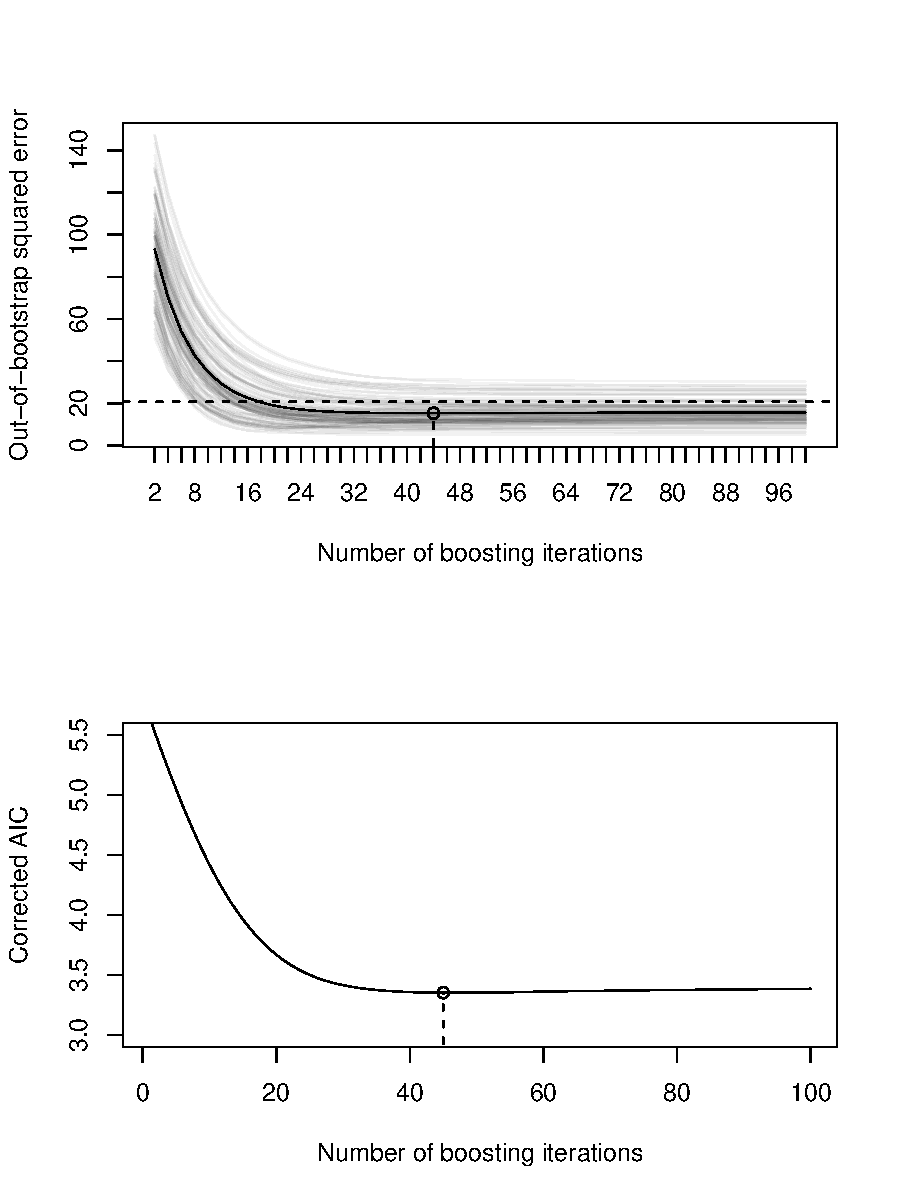
\includegraphics{figures/bodyfat_glmboost-bodyfat-oob-plot.pdf}
\caption{\Robject{bodyfat} data: Out-of-bootstrap squared error for varying number of 
         boosting iterations $m_\text{stop}$ (top). The dashed horizontal line
         depicts the out-of-bootstrap error of the linear model 
         for the pre-selected variables \Robject{hipcirc}, \Robject{kneebreadth} 
         and \Robject{anthro3a} fitted via ordinary least squares. 
         The lower part show the corrected AIC criterion.
         \label{bodyfat-oob-plot}}
\end{center}
\end{figure}


We notice that most covariates have been used for fitting
and thus no extensive variable selection was performed in the above model. 
Thus, we need to investigate how many boosting iterations are appropriate. Resampling
methods such as cross-validation or the bootstrap can be used to study the 
empirical risk for a varying number of boosting iterations. The out-of-bootstrap mean 
squared error for $100$ bootstrap samples is depicted in the upper part of 
Figure~\ref{bodyfat-oob-plot}. The plot
leads to the impression that approximately $m_\text{stop} = 44$ would be a sufficient
number of boosting iterations.
In Section~\ref{subsec.stopping}, a corrected version of the Akaike
information criterion (AIC) is proposed for determining the optimal number
of boosting iterations. This criterion attains its 
minimum for
\begin{Schunk}
\begin{Sinput}
R> mstop(aic <- AIC(bf_glm))
\end{Sinput}
\begin{Soutput}
[1] 45
\end{Soutput}
\end{Schunk}
boosting iterations, see the bottom part of
Figure~\ref{bodyfat-oob-plot} in addition.

The coefficients of the boosted linear model with 
$m_\text{stop} = 45$ 
boosting iterations are
\begin{Schunk}
\begin{Sinput}
R> coef(bf_glm[mstop(aic)])
\end{Sinput}
\begin{Soutput}
 (Intercept)          age    waistcirc      hipcirc 
   0.0000000    0.0023271    0.1893046    0.3488781 
elbowbreadth  kneebreadth     anthro3a     anthro3b 
   0.0000000    1.5217686    3.3268603    3.6051548 
    anthro3c      anthro4 
   0.5043133    0.0000000 
attr(,"offset")
[1] 30.783
\end{Soutput}
\end{Schunk}
and thus only 7 covariates have been selected for the final
model (intercept equal to zero occurs here for mean centered response and
predictors and hence, 
%TORSTEN: PLEASE CHECK
$n^{-1} \sum_{i=1}^n Y_i = 30.783$
%TORSTEN
is the intercept in the uncentered model). Note that   
the variables \Robject{hipcirc}, \Robject{kneebreadth} and
\Robject{anthro3a}, which 
we have used for fitting a simple linear model at the beginning of this
paragraph, have been selected by the boosting algorithm as well. 


 

\paragraph{Illustration: Prediction of Total Body Fat (cont.)}

	%%%% DON'T EDIT THIS FILE

\setkeys{Gin}{width = 0.97\textwidth}
Being more flexible than the linear model which we fitted to the
\Robject{bodyfat} data in Section~\ref{subsec.compLS}, we estimate an additive
model using the \Rcmd{gamboost} function from \Rpackage{mboost} (first with
pre-specified $m_\text{stop} = 100$ 
boosting iterations, $\nu = 0.1$ and squared error loss):
\begin{Schunk}
\begin{Sinput}
R> bf_gam <- gamboost(bffm, data = cbodyfat)
\end{Sinput}
\end{Schunk}
The degrees of freedom for the smoothing splines, which are utilized as
base learners here, 
can be defined by the \Rcmd{dfbase} argument, defaulting to $4$. 

We can estimate the number of boosting iterations $m_\text{stop}$
using the corrected AIC criterion described in
Section~\ref{subsec.stopping}
(see Figure~\ref{bodyfat-gamboost-AIC}) via
\begin{Schunk}
\begin{Sinput}
R> mstop(aic <- AIC(bf_gam))
\end{Sinput}
\begin{Soutput}
[1] 46
\end{Soutput}
\begin{Sinput}
R> bf_gam <- bf_gam[mstop(aic)]
\end{Sinput}
\end{Schunk}
Similar to the linear regression model, the partial contributions of the covariates
can be extracted from the boosting fit. For the most important variables, 
the partial fits are given in Figure~\ref{bodyfat-gamboost-plot} showing some 
slight non-linearity for \Robject{hipcirc} and \Robject{kneebreadth}.

\begin{figure}
\begin{center}
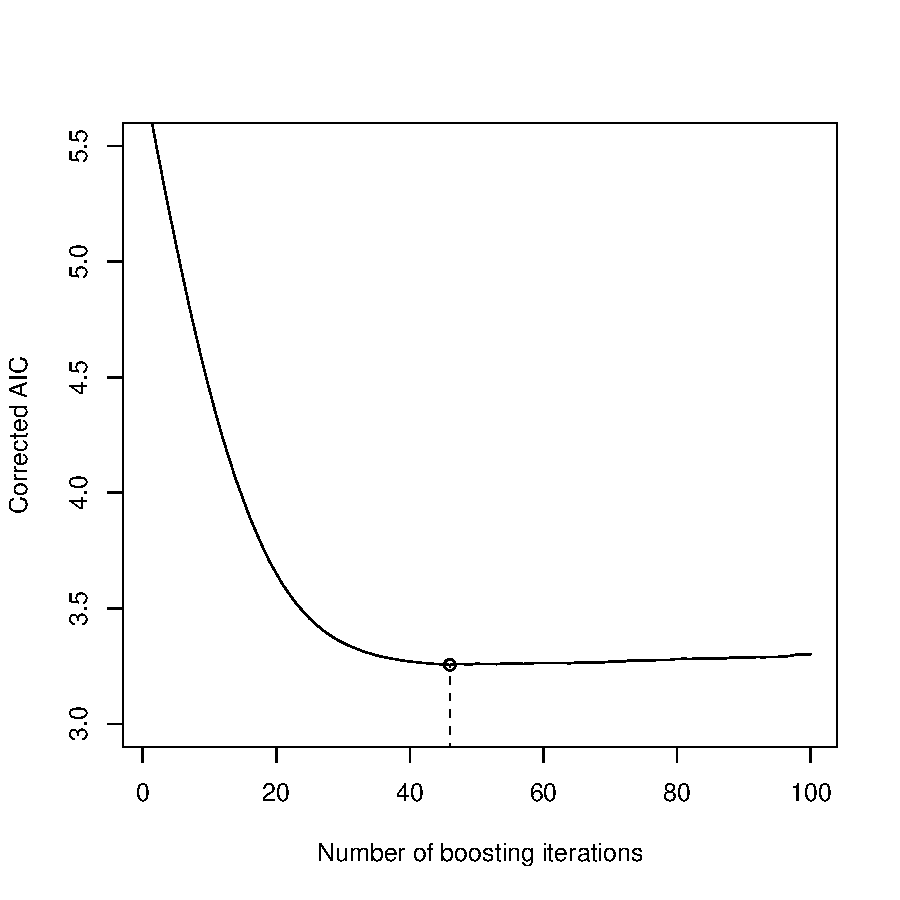
\includegraphics{figures/BH-bodyfat-gamboost-AIC}
\caption{\Robject{bodyfat} data: Corrected AIC as a function of the number of 
boosting iterations $m_\text{stop}$ 
for fitting an additive model via \Rcmd{gamboost}. \label{bodyfat-gamboost-AIC}}
\end{center}
\end{figure}


\begin{figure}
\begin{center}
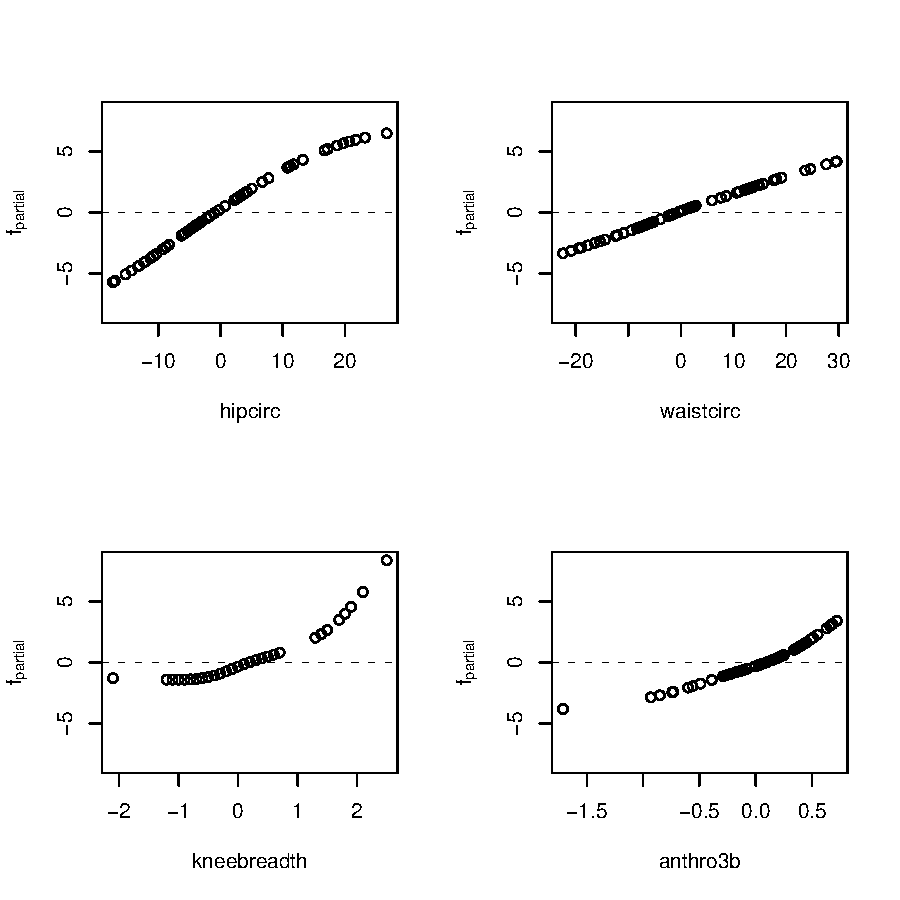
\includegraphics{figures/BH-bodyfat-gamboost-plot}
\caption{\Robject{bodyfat} data: Partial contributions of four covariates in an additive model. 
         \label{bodyfat-gamboost-plot}}
\end{center}
\end{figure}

 

\paragraph{Illustration: Prediction of Total Body Fat (cont.)}

	%%%% DON'T EDIT THIS FILE

\setkeys{Gin}{width = 0.97\textwidth}
Such transformation defined in terms
of fractional polynomials for estimating a linear model can be used with
the \Rcmd{glmboost} function 
\citep[an implementation of the original fractional polynomials approach is
available in package \Rpackage{mfp}, see][]{pkg:mfp,Sauerbreietal2006},
where the model formula performs the computations of all transformations by 
means of the \Rcmd{FP} (fractional polynomials) function. First, we scale
each covariate to the interval $[1,2]$ and then fit the complex linear model
by using the \Rcmd{glmboost} function with initial $m_\text{stop} = 3000$ boosting
iterations:
\begin{Schunk}
\begin{Sinput}
R> tbodyfat <- bodyfat
R> tbodyfat[indep] <- lapply(bodyfat[indep], function(x) {
         x <- x - min(x)
         x/max(x) + 1
     })
R> fpfm <- as.formula(paste("DEXfat ~ ", paste("FP(", 
         indep, ")", collapse = "+")))
R> fpfm
\end{Sinput}
\begin{Soutput}
DEXfat ~ FP(age) + FP(waistcirc) + FP(hipcirc) + FP(elbowbreadth) + 
    FP(kneebreadth) + FP(anthro3a) + FP(anthro3b) + FP(anthro3c) + 
    FP(anthro4)
\end{Soutput}
\begin{Sinput}
R> bf_fp <- glmboost(fpfm, data = tbodyfat, control = boost_control(mstop = 3000))
R> mstop(aic <- AIC(bf_fp))
\end{Sinput}
\begin{Soutput}
[1] 2480
\end{Soutput}
\end{Schunk}
The corrected AIC criterion (see Section~\ref{subsec.stopping}) suggests to
stop after $m_\text{stop} = 2480$ 
boosting iterations and the final model selects
$21$ (transformed) predictor
variables. Again, the partial 
contributions of each of the 9 original covariates can be computed
easily and are shown  
(for the same variables as in Figure~\ref{bodyfat-gamboost-plot}) in 
Figure~\ref{bodyfat-fpboost-plot}. Note that the depicted functional
relationship derived 
from the multivariate fractional polynomial model
(Figure~\ref{bodyfat-fpboost-plot}) is qualitatively the same as the one
derived from the additive model   
(Figure~\ref{bodyfat-gamboost-AIC}). 

\begin{figure}
\begin{center}
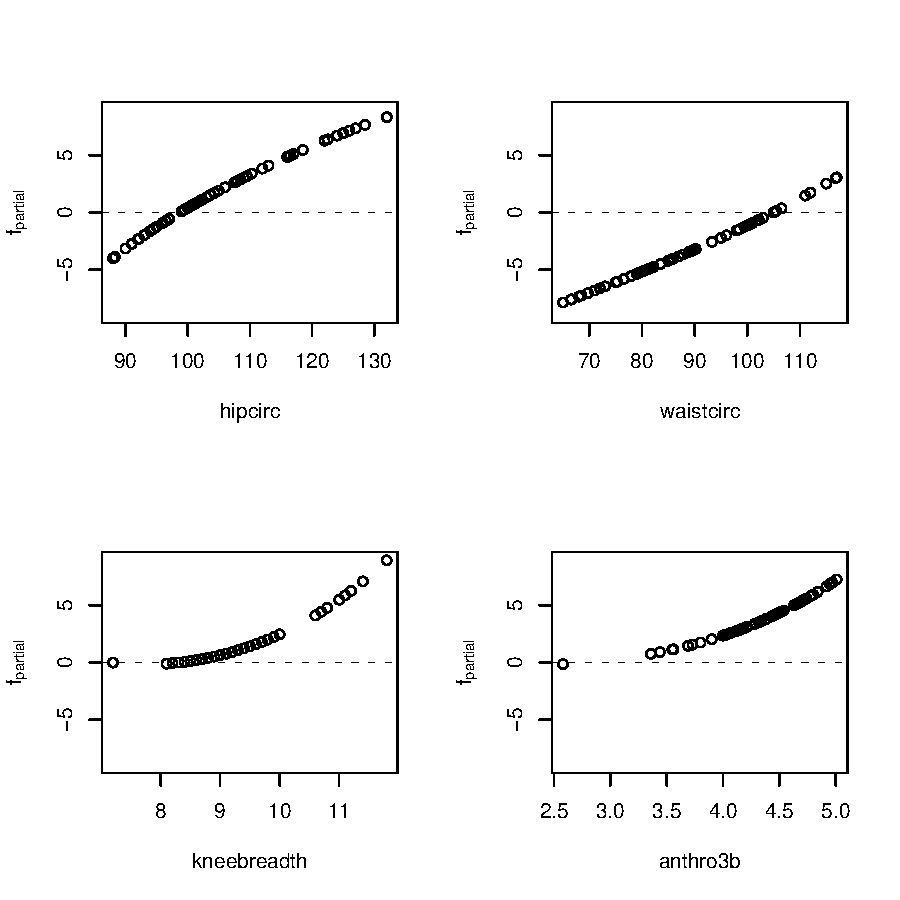
\includegraphics{figures/BH-bodyfat-fpboost-plot}
\caption{\Robject{bodyfat} data: Partial fits for a linear model including 
fractional polynomials. \label{bodyfat-fpboost-plot}}
\end{center}
\end{figure}



\paragraph{Illustration: Wisconsin Prognostic Breast Cancer}

	%%%% DON'T EDIT THIS FILE

\setkeys{Gin}{width = 0.97\textwidth}
Prediction models for recurrence events in breast cancer patients 
based on covariates which have been computed from a digitized image of a
fine needle aspirate of breast tissue (those measurements describe
characteristics of the cell nuclei present in the image) have been studied
by \citet{street1995} \citep[the data is part of the UCI repository][]{uci1998}.

We first analyse this data as a binary prediction problem 
(recurrence vs. non-recurrence) and later in Section~\ref{sec.survival} 
by means of survival models. Again, we are faced with lots of potential covariates ($p = 32$) 
for a limited number of observations without missing values 
($n = 194$) and variable selection is an issue. We can choose a classical logistic regression model 
via AIC in a stepwise algorithm as follows (after centering the covariates)
\begin{Schunk}
\begin{Sinput}
R> wpbc2 <- wpbc[complete.cases(wpbc), colnames(wpbc) != 
         "time"]
R> indep <- names(wpbc2)[names(wpbc2) != "status"]
R> wpbc2[indep] <- lapply(wpbc2[indep], function(x) x - 
         mean(x))
R> wpbc_step <- step(glm(status ~ ., data = wpbc2, 
         family = binomial()), trace = 0)
\end{Sinput}
\end{Schunk}
The final model consists of 16 parameters with
\begin{Schunk}
\begin{Sinput}
R> logLik(wpbc_step)
\end{Sinput}
\begin{Soutput}
'log Lik.' -80.13 (df=16)
\end{Soutput}
\begin{Sinput}
R> AIC(wpbc_step)
\end{Sinput}
\begin{Soutput}
[1] 192.26
\end{Soutput}
\end{Schunk}
and we want to compare this model to a logistic regression model fitted via gradient boosting. 
We simply select the \Robject{Binomial} family (with default offset of $1/2 \log(p / (1 - p))$, 
where $p$ is the proportion of recurrences) and start with initial 
$m_\text{stop} = 500$ boosting iterations
\begin{Schunk}
\begin{Sinput}
R> wpbc_glm <- glmboost(status ~ ., data = wpbc2, 
         family = Binomial(), control = boost_control(mstop = 500))
\end{Sinput}
\end{Schunk}
The negative binomial log-likelihood is
\begin{Schunk}
\begin{Sinput}
R> logLik(wpbc_glm)
\end{Sinput}
\begin{Soutput}
[1] -89.964
\end{Soutput}
\end{Schunk}
and the classical AIC criterion suggests to stop after
\begin{Schunk}
\begin{Sinput}
R> aic <- AIC(wpbc_glm, "classical")
R> aic
\end{Sinput}
\begin{Soutput}
[1] 198.45
Optimal number of boosting iterations: 260 
Degrees of freedom (for mstop = 260): 7.035 
\end{Soutput}
\end{Schunk}
boosting iterations. 
%%Again, we want to investigate the out-of-bootstrap performance
%%of the boosted logistic regression model. Figure~\ref{wpbc-benchmarks-plot} depicts the
%%out-of-bootstrap (positive) binomial log-likelihood, standardized with 
%%the number of out-of-bootstrap observations, for varying number of boosting iterations $m_\text{stop}$. 
%%\begin{figure}
%%\begin{center}
%%<<wpbc-benchmarks-plot, echo = FALSE, fig = TRUE>>=
%%load(system.file("cache/wpbc_benchmarks.rda", package = "mboost"))
%%grid <- seq(from = 5, to = 500, by = 5)
%%plot(c(0, grid[-1] - 5), -colMeans(boob), type = "b", 
%%     ylab = "Log-Likelihood / n",
%%     xlab = "Number of Boosting Iterations")
%%mopt <- grid[which.max(colMeans(boob))]
%%@
%%\caption{\Robject{wpbc} data: Out-of-bootstrap (positive) binomial 
%%    log-likelihood. \label{wpbc-benchmarks-plot}}
%%\end{center}
%%\end{figure}
We now restrict the number of boosting iterations to 
$m_\text{stop} = 260$ via
\begin{Schunk}
\begin{Sinput}
R> wpbc_glm <- wpbc_glm[mstop(aic)]
R> logLik(wpbc_glm)
\end{Sinput}
\begin{Soutput}
[1] -92.189
\end{Soutput}
\begin{Sinput}
R> coef(wpbc_glm)[abs(coef(wpbc_glm)) > 0]
\end{Sinput}
\begin{Soutput}
     (Intercept)     mean_texture    mean_symmetry 
     -3.0110e-02      -2.4215e-02      -3.3878e+00 
 mean_fractaldim       SE_texture     SE_perimeter 
     -2.0321e+01      -2.6603e-02       4.0908e-02 
  SE_compactness     SE_concavity SE_concavepoints 
      7.0280e+00      -4.6303e+00      -1.5737e+01 
     SE_symmetry     worst_radius  worst_perimeter 
      2.8601e+00       1.7777e-02       1.2639e-03 
      worst_area worst_smoothness            tsize 
      1.5854e-04       8.8372e+00       3.1014e-02 
          pnodes 
      2.5981e-02 
\end{Soutput}
\end{Schunk}
(because of using the offset-value $\hat{f}^{[0]}$, we have to add the value
$\hat{f}^{[0]}$ to the reported intercept estimate above for the logistic
regression model) and we then can
extract the fitted conditional probabilities  
\begin{Schunk}
\begin{Sinput}
R> f <- fitted(wpbc_glm)
R> p <- exp(f)/(exp(f) + exp(-f))
\end{Sinput}
\end{Schunk}
which are depicted by a conditional density plot in 
Figure~\ref{wpbc-glmboost-prob-plot}.

\begin{figure}
\begin{center}
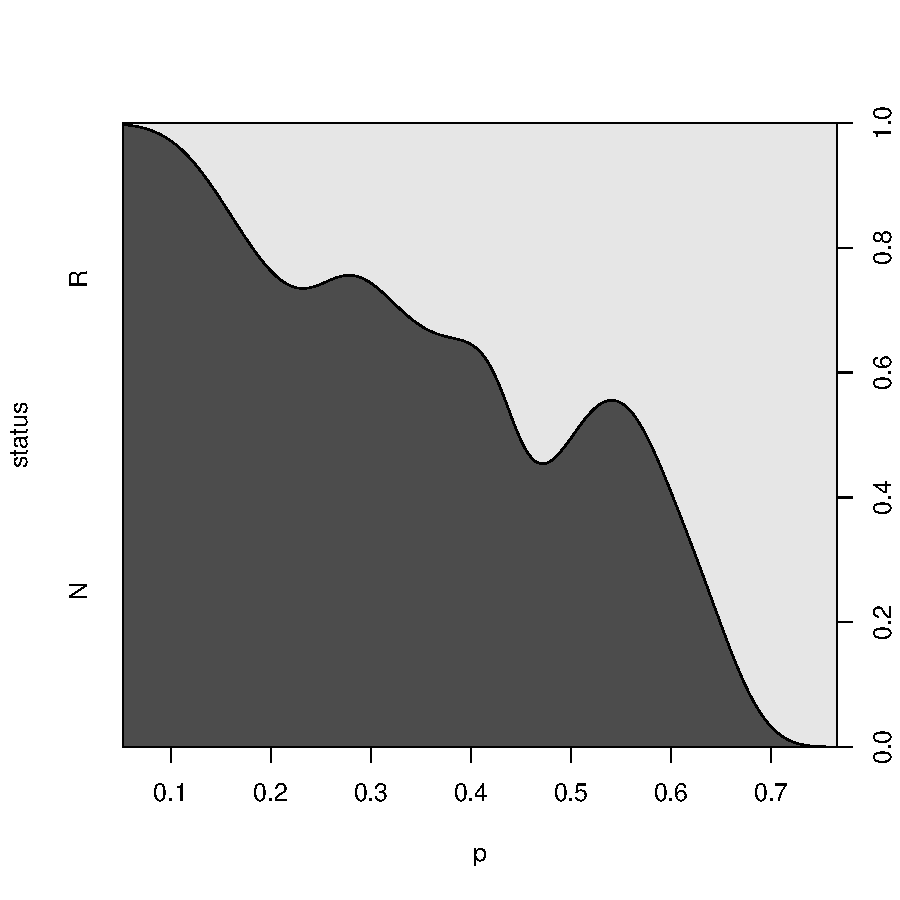
\includegraphics{figures/BH-wpbc-glmboost-prob-plot}
\caption{\Robject{wpbc} data: Conditional density plot of the fitted 
         probabilities of recurrence / non-recurrence. \label{wpbc-glmboost-prob-plot}}
\end{center}
\end{figure}

A generalized additive model adds more flexibility to the regression function but is still
interpretable. We fit a logistic additive model to the \Robject{wpbc} data as follows:
\begin{Schunk}
\begin{Sinput}
R> wpbc_gam <- gamboost(status ~ ., data = wpbc2, 
         family = Binomial())
R> mopt <- mstop(aic <- AIC(wpbc_gam, "classical"))
R> aic
\end{Sinput}
\begin{Soutput}
[1] 196.33
Optimal number of boosting iterations: 84 
Degrees of freedom (for mstop = 84): 13.754 
\end{Soutput}
\end{Schunk}
This model selected $16$ out of $32$
covariates. The partial contributions of the four most important variables
are depicted in  
Figure~\ref{wpbc-gamboost-plot} indicating a remarkable degree of non-linearity.
\begin{figure}
\begin{center}
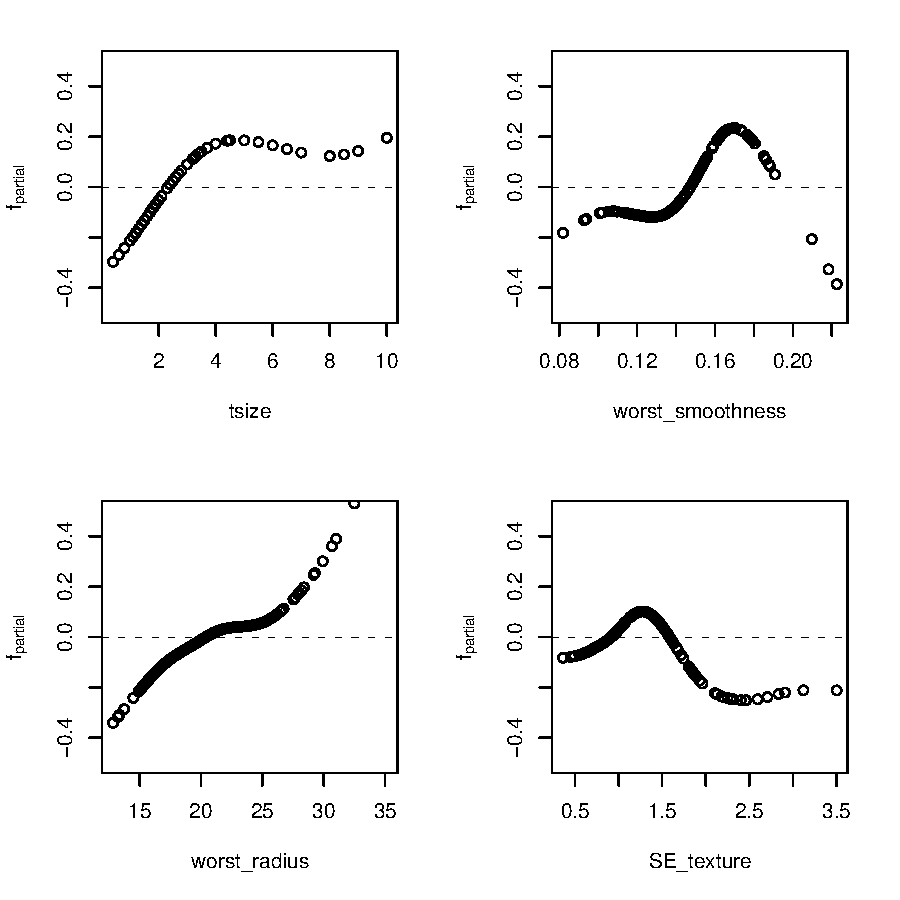
\includegraphics{figures/BH-wpbc-gamboost-plot}
\caption{\Robject{wpbc} data: Partial contributions of four selected 
    covariates in an additive logistic model.
    \label{wpbc-gamboost-plot}}
\end{center}
\end{figure}



\paragraph{Illustration: Wisconsin Prognostic Breast Cancer (cont.)}         

	%%%% DON'T EDIT THIS FILE

\setkeys{Gin}{width = 0.97\textwidth}Instead of the binary response variable describing the recurrence status we
make use of the additionally available time information for modeling
the time to recurrence, i.e., all observations with non-recurrence are censored.
First, we calculate IPC weights and center the covariates
\begin{Schunk}
\begin{Sinput}
R> iw <- IPCweights(Surv(wpbc$time, wpbc$status == 
         "R"))
R> wpbc3 <- wpbc[, colnames(wpbc) != "status"]
R> indep <- names(wpbc3)[names(wpbc3) != "time"]
R> wpbc3[indep] <- lapply(wpbc3[indep], function(x) x - 
         mean(x, na.rm = TRUE))
\end{Sinput}
\end{Schunk}
and fit a weighted linear model by boosting with componentwise linear
weighted least squares as base procedure: 
\begin{Schunk}
\begin{Sinput}
R> wpbc_surv <- glmboost(log(time) ~ ., data = wpbc3, 
         control = boost_control(mstop = 500), weights = iw)
R> mstop(aic <- AIC(wpbc_surv))
\end{Sinput}
\begin{Soutput}
[1] 122
\end{Soutput}
\begin{Sinput}
R> wpbc_surv <- wpbc_surv[mstop(aic)]
\end{Sinput}
\end{Schunk}
The following variables have been selected for fitting 
\begin{Schunk}
\begin{Sinput}
R> names(coef(wpbc_surv)[abs(coef(wpbc_surv)) > 0])
\end{Sinput}
\begin{Soutput}
 [1] "mean_radius"         "mean_texture"       
 [3] "mean_perimeter"      "mean_smoothness"    
 [5] "mean_symmetry"       "SE_texture"         
 [7] "SE_smoothness"       "SE_concavepoints"   
 [9] "SE_symmetry"         "worst_concavepoints"
\end{Soutput}
\end{Schunk}
and the fitted values are 
depicted in Figure~\ref{wpbc-glmboost-censored-fit}, showing a reasonable model fit.

\begin{figure}
\begin{center}
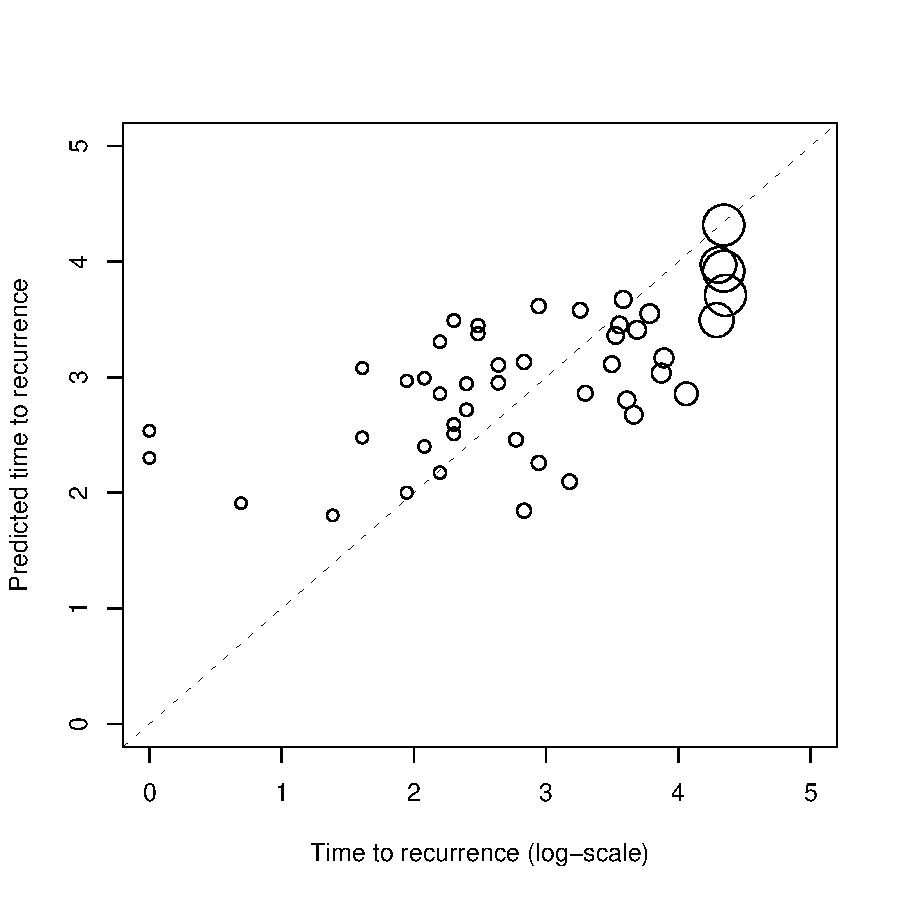
\includegraphics{figures/BH-wpbc-glmboost-censored-fit}
\caption{\Robject{wpbc} data: Fitted values of a weighted linear model taking both time to recurrence and
    censoring information into account. The radius of the circles is proportional to the
    IPC weight of the corresponding observation, censored observations with IPC weight zero
    are not plotted. \label{wpbc-glmboost-censored-fit}}
\end{center}
\end{figure}

\clearpage

\bibliographystyle{plainnat}
\bibliography{boost}

\end{document}
